%----------------------------------------------------------------------------------------
%	PACKAGES AND THEMES
%----------------------------------------------------------------------------------------
\documentclass[xcolor=dvipsnames]{beamer}
\usetheme{Simple}

\usepackage{hyperref}
\usepackage{graphicx} % Allows including images
\usepackage{booktabs} % Allows the use of \toprule, \midrule and \bottomrule in tables

\usepackage{amssymb}
\usepackage[english]{babel}

%----------------------------------------------------------------------------------------
%	TITLE PAGE
%----------------------------------------------------------------------------------------

% The title
\title[Bayesian Adaptive Methods Review]{A First Look at Bayesian Adaptive Methods}
\subtitle{}

\author[FB] {Fan Bu}
% \institute[]
% {
% }
\date{October 12, 2021}


%----------------------------------------------------------------------------------------
%	PRESENTATION SLIDES
%----------------------------------------------------------------------------------------

\begin{document}

\begin{frame}
    % Print the title page as the first slide
    \titlepage
\end{frame}

\begin{frame}{Overview}
    % Throughout your presentation, if you choose to use \section{} and \subsection{} commands, these will automatically be printed on this slide as an overview of your presentation
    \tableofcontents
\end{frame}

%------------------------------------------------
\section{Basics of Bayesian hypothesis testing}
%------------------------------------------------

\begin{frame}
    \Huge{\centerline{Basics of Bayesian hypothesis testing}}
\end{frame}

\begin{frame}{Basic setup}
\begin{itemize}
    \item Observe data $X$  $ \sim p(x \mid \theta)$ (data model) w/. parameter $\theta$
    \item Wish to test 
    \begin{equation*}
     H_0: \theta \in \Theta_0 \qquad \text{ v.s. } \qquad H_1: \theta \in \Theta_1
     \end{equation*}
     \pause
     \item prior beliefs about the hypotheses: $p := P(H_0)$ (then $1-p = P(H_1)$)
     \item priors for $\theta$: $\pi_i$ under $H_i$ ($i=0,1$)
\end{itemize}
    
\end{frame}

\begin{frame}{Evidence checking via posterior inference}
\begin{itemize}
    \item posterior distribution for $\theta$ under $H_i$ ($i=0,1$):
    \begin{equation}
    p(\theta \mid x, H_i) = \frac{p(x \mid \theta) \pi_i(\theta)}{m_i(x)};
    \end{equation}
    \item $m_i(x) = \int p(x \mid \theta) \pi_i(\theta) d\theta$: marginal distribution of data $X$ (or data evidence) under $H_i$. 
    \pause
    \item posterior odds in favor of $H_0$:
    \begin{equation}
    \frac{P(H_0 \mid x)}{P(H_1 \mid x)} = \frac{m_0(x) p}{m_1(x) (1-p)} = \frac{m_0(x)}{m_1(x)} \frac{p}{1-p};
    \end{equation}
    \pause
    \item Bayes factor (posteriors odds when $p=1/2$):
    \begin{equation}
    \label{eq:bayes-factor}
    BF_{01} = \frac{m_0(x)}{m_1(x)}.
    \end{equation}
\end{itemize}
    
\end{frame}

\begin{frame}{Evidence checking (Cont'd)}
\begin{itemize}
    \item For simple v.s. simple hypothesis testing, BF is same as likelihood ratio:
    \begin{equation}
    BF_{01} = \frac{p(x \mid \theta_0)}{p(x \mid \theta_1)}.
    \end{equation}
    \pause
    \item With threshold $A$, would reject $H_0$ if $BF_{01} < A$;
    \item Or, equivalently, with threshold $\delta_L$, reject $H_0$ if $P(H_0 \mid x) < \delta_L$.
\end{itemize}
\end{frame}

%------------------------------------------------
\section{Bayesian sequential testing}
%------------------------------------------------

\begin{frame}
    \Huge{\centerline{Bayesian sequential testing}}
\end{frame}

\begin{frame}{Bayesian analysis is intrinsically sequential}
A current ``posterior'' can become the ``prior'' for future inference. 
\only<1>{
\begin{figure}
    \centering
    %\vspace{-0.1in}
    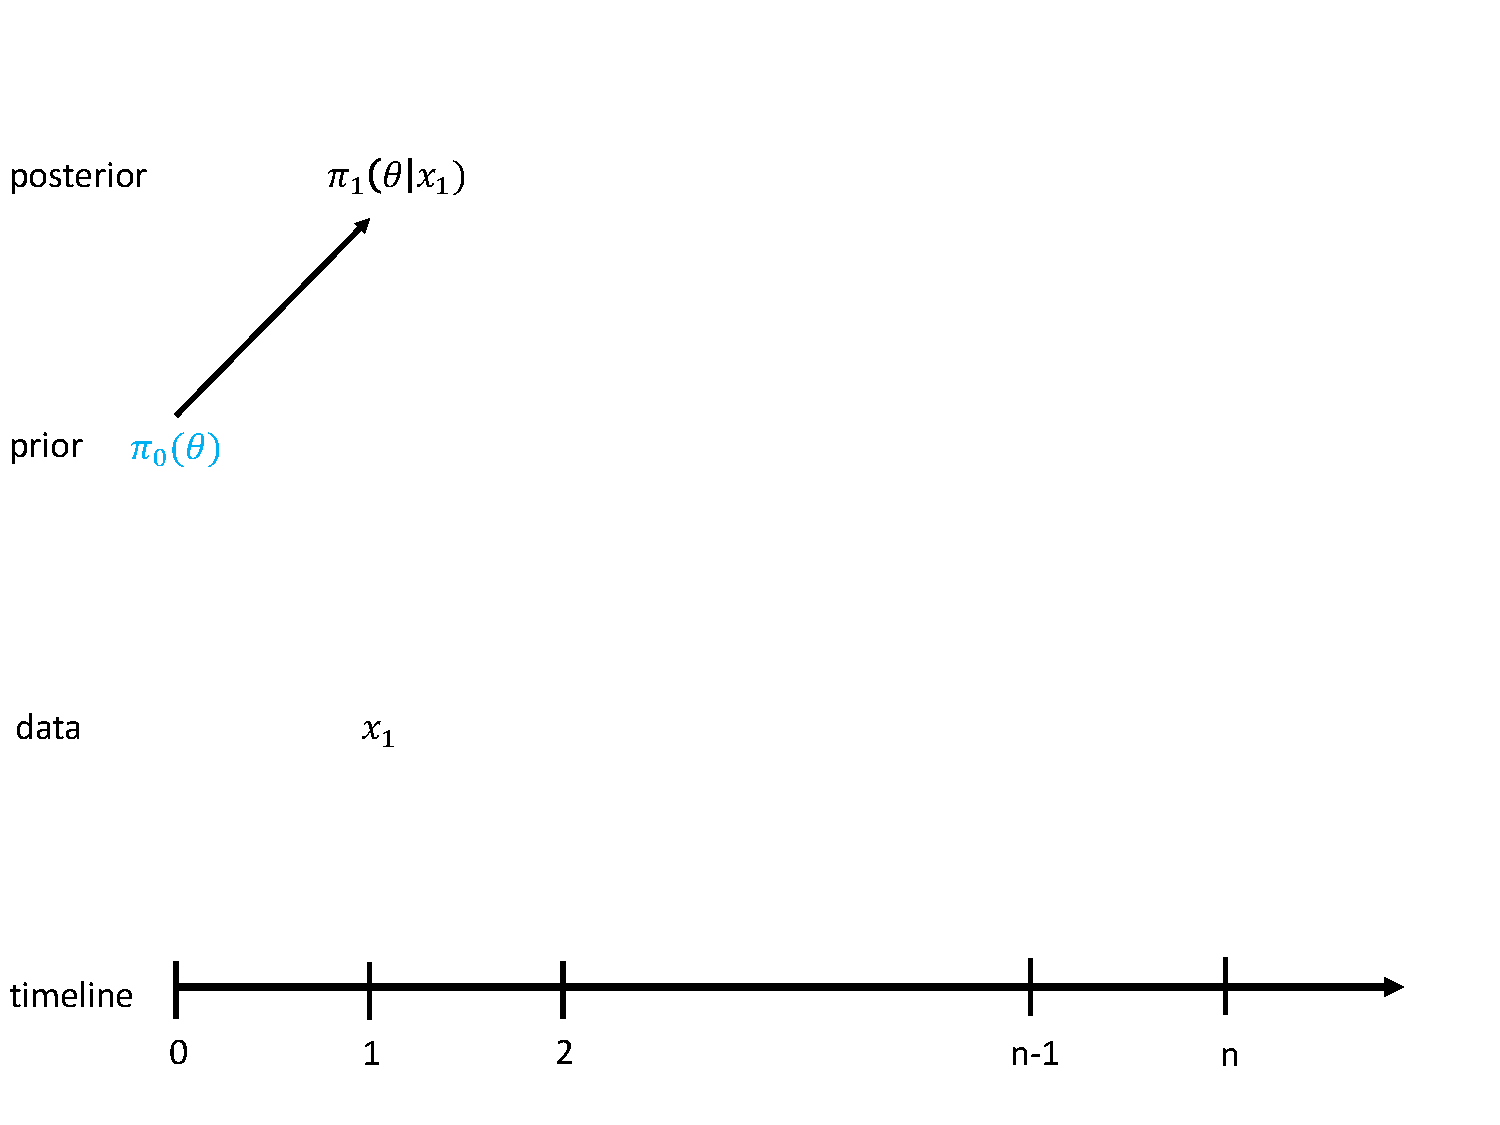
\includegraphics[width=0.87\textwidth, page=1, trim=0 0 0.5in 0.5in, clip]{figures/Bayesian_sequential_updating.pdf}
\end{figure}
}
\only<2>{
\begin{figure}
    \centering
    %\vspace{-0.1in}
    \includegraphics[width=0.87\textwidth, page=2, trim=0 0 0.5in 0.5in, clip]{figures/Bayesian_sequential_updating.pdf}
\end{figure}
}
\only<3>{
\begin{figure}
    \centering
    %\vspace{-0.1in}
    \includegraphics[width=0.87\textwidth, page=3, trim=0 0 0.5in 0.5in, clip]{figures/Bayesian_sequential_updating.pdf}
\end{figure}
}
\only<4>{
\begin{figure}
    \centering
    %\vspace{-0.1in}
    \includegraphics[width=0.87\textwidth, page=4, trim=0 0 0.5in 0.5in, clip]{figures/Bayesian_sequential_updating.pdf}
\end{figure}
}

\end{frame}

\begin{frame}{How it usually works}
Given thresholds $B \geq 1 \geq A$, with Bayes factor $BF_{01}^{(n)}$ acquired at step $n$ \footnote{See, for example, \cite{barnard1946sequential,wetherill1961bayesian,berger1994unified,berger1988likelihood,berger1997unified,berger1999simultaneous}.}:
\begin{itemize}
	\item if $BF_{01}^{(n)} > B$, stop the study and accept $H_0$;
	\item if $A < BF_{01}^{(n)} < B$, continue the study;
	\item  if $BF_{01}^{(n)} < A$, stop the study and reject $H_0$.
\end{itemize}

\pause
\vspace{0.2in}
Of course, we can make decisions based on the posterior probability $P(H_0 \mid x)$ or $P(H_1 \mid x)$ with specified thresholds (e.g., \cite{cornfield1966bayesian}).


    
\end{frame}


%------------------------------------------------
\section{Examples of Bayesian adaptive methods application}
%------------------------------------------------

\begin{frame}
    \Huge{Examples of Bayesian adaptive methods application}
\end{frame}  

\begin{frame}{The setup}
\begin{itemize}
    \item Compare effect $\theta$ (e.g., log relative risk) with baseline $\theta_0$:
    \begin{equation*}
    H_0: \theta \leq \theta_0 \qquad \text{ v.s. } \qquad H_1: \theta > \theta_0.
    \end{equation*}
    \pause
    \item Or, consider a ``minimal practical increase'' $\delta$:
    \begin{equation*}
    H_0: \theta \leq \theta_0 + \delta \qquad \text{ v.s. } \qquad H_1: \theta > \theta_0 + \delta.
    \end{equation*}
\end{itemize}
    
\end{frame}

\begin{frame}{Binary decisions}
\begin{itemize}
    \item Specify lower and upper probability bounds $\delta_L$ and $\delta_U$;
    \item \textbf{Early stopping for signal} if $P(H_1 \mid x) > \delta_U$;
    \item \textbf{Early stopping for futility} if $P(H_1 \mid x) < \delta_L$. 
    \item Common choice: $\delta_L = 0.05, 0.1$, $\delta_U = 0.8, 0.95$, OR calibrated through simulations.
    \footnote{See, for example, \cite{thall1995bayesian,smith2006implementation,zhou2008bayesian,berry2010bayesian,li2020bayesian}, etc.}
\end{itemize}
    
\end{frame}

\begin{frame}{Non-binary decisions}
We can draw different conclusions about the strength of evidence in support of either hypothesis. 

\vspace{0.2in}
Decisions based on $BF_{10}$ (Bayes factor in favor of $H_1$)
\cite{jeffreys1998theory,kass1995bayes,schonbrodt2017sequential}:
\begin{itemize}
	\item  $1 < BF_{10} < 3$: anecdotal evidence
	\item  $3 < BF_{10} < 10$: moderate evidence
	\item $10 <	BF_{10} < 30$: strong evidence
	\item $BF_{10} > 30$ very strong evidence. 
\end{itemize}
    
\end{frame}

\begin{frame}{Non-binary decisions (Cont'd) - zone method}
Or, given an indifference zone $[\delta_L, \delta_U]$,  make decisions based on credible interval for $\Delta = \theta - \theta_0$ \cite{berry2010bayesian}. 

\begin{figure}
    \centering
    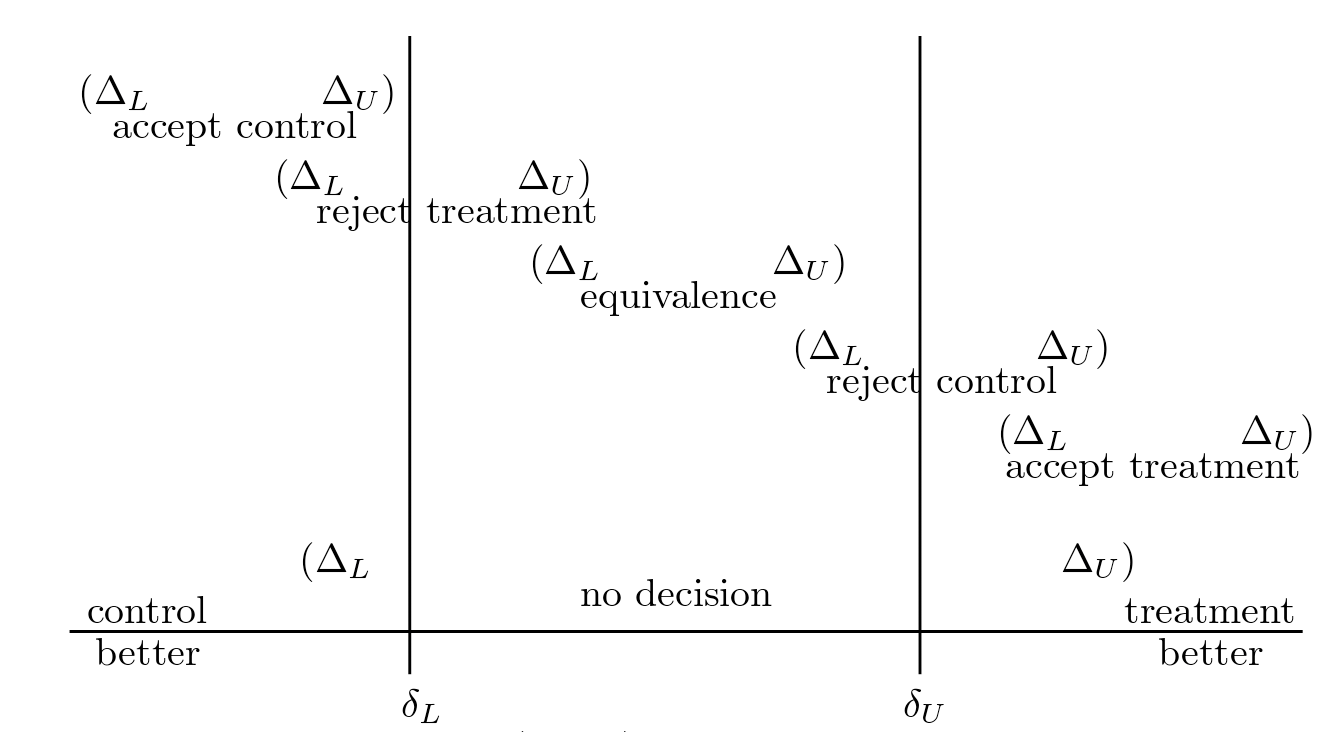
\includegraphics[width=0.88\textwidth]{figures/Bayeisan-zone-method-stopping-rules.png}
\end{figure}
\end{frame}


%------------------------------------------------
\section{Methodological gaps BST can address}
%------------------------------------------------

\begin{frame}
    \Huge{\centerline{Advantages and methodological gaps}}
\end{frame}  

\begin{frame}{Advantages}
\begin{itemize}
    \item Easy to incorporate historical data through priors:
    \begin{itemize}
        \item e.g., historical adverse event incidence rate $1\%$, then can use $\text{Beta}(1,99)$ prior for incidence rate $\theta$
        \item can ``discount'' prior to address temporal changes \cite{west2006bayesian}
    \end{itemize}
    \pause
    \item Can test multiple hypotheses (e.g., detect multiple safety signals) simultaneously \cite{gopalan1998bayesian,berry1999bayesian,scott2006exploration,labbe2007multiple,guo2010multiplicity,kachiashvili2012sensitivity,kachiashvili2013conditional,kachiashvili2014methods,berger2013statistical}
\end{itemize}
    
\end{frame}

\begin{frame}{Advantages}
\begin{itemize}
    \item Can incorporate model selection/averaging within the Bayesian framework (e.g., \cite{raftery1995bayesian,wasserman2000bayesian,chipman2001practical,stephan2009bayesian,wathen2008bayesian,senarathne2020laplace})
    \item Non-violation of \textbf{the likelihood principle}:
    \begin{itemize}
        \item ``Given a statistical model, all information relavent to inferences about model parameters $\theta$ is contained in the likelihood function $L(\theta ; x)$'';
        \item ``If two likelihood functions $L_1(\theta ; x)$ and $L_2(\theta ; x)$ are proportional then they contain same information about $\theta$''.
        \item Conclusions about a study shouldn't depend on how we look at the data or how we decide when to stop - frequentist sequential analysis clearly violates this
        \item Bayesian analysis respects the likelihood principle
    \end{itemize}
\end{itemize}
    
\end{frame}

\begin{frame}{Potential challenges}
\begin{itemize}
    \item Calibration of the thresholds
    \begin{itemize}
        \item No universal rule (like $\alpha = 0.05$)
        \item Theoretical results for matching frequentist error rate bounds available for simple models (e.g.,\cite{berger1994unified, cornfield1966bayesian})
        \pause
        \item Can use simulation-based or data-driven calibration (negative/positive controls utilizing OHDSI network) to satisfy frequentist operating characteristics requirements 
    \end{itemize}
\end{itemize}
    
\end{frame}

\begin{frame}{Potential challenges}
\begin{itemize}
    \item Model-free or likelihood-free cases
    \begin{itemize}
        \item When a data model cannot be be easily specified or a likelihood function doesn't exist;
        \item Traditional Bayesian approach can't be applied, but generalized Bayesian methods for likelihood-free or loss-function-based inference might be employed (e,g., \cite{turner2014generalized, lyddon2019general, bissiri2016general}).
    \end{itemize}
\end{itemize}
    
\end{frame}


\begin{frame}
    \Huge{\centerline{Thank you!}}
\end{frame}

%----------------------------------------------------------------------------------------

\begin{frame}
\Huge{\centerline{Likelihood Principle Examples}}
\end{frame}

\begin{frame}[plain]
    \begin{figure}
        \centering
        \includegraphics[page=6, width=0.9\textwidth, trim=0 0.45in 0 0.6in, clip]{figures/History-Lecture 7.pdf}
    \end{figure}
    
\footnotesize{Credit: James Berger}
\end{frame}

\begin{frame}[plain]
    \begin{figure}
        \centering
        \includegraphics[page=7, width=0.9\textwidth, trim=0 0.45in 0 0.6in, clip]{figures/History-Lecture 7.pdf}
    \end{figure}
    
\footnotesize{Credit: James Berger}
\end{frame}

\begin{frame}[plain]
    \begin{figure}
        \centering
        \includegraphics[page=8, width=0.9\textwidth, trim=0 0.45in 0 0.6in, clip]{figures/History-Lecture 7.pdf}
    \end{figure}
    
\footnotesize{Credit: James Berger}
\end{frame}

\begin{frame}[plain]
    \begin{figure}
        \centering
        \includegraphics[page=9, width=0.9\textwidth, trim=0 0.45in 0 0.6in, clip]{figures/History-Lecture 7.pdf}
    \end{figure}
    
\footnotesize{Credit: James Berger}
\end{frame}

\begin{frame}[plain]
    \begin{figure}
        \centering
        \includegraphics[page=10, width=0.9\textwidth, trim=0 0.45in 0 0.6in, clip]{figures/History-Lecture 7.pdf}
    \end{figure}
    
\footnotesize{Credit: James Berger}
\end{frame}

\begin{frame}[plain]
    \begin{figure}
        \centering
        \includegraphics[page=11, width=0.9\textwidth, trim=0 0.45in 0 0.6in, clip]{figures/History-Lecture 7.pdf}
    \end{figure}
    
\footnotesize{Credit: James Berger}
\end{frame}

\begin{frame}[allowframebreaks]
        \frametitle{References}
        \bibliographystyle{amsalpha}
        \bibliography{ref.bib}
\end{frame}
\end{document}